\begin{figure}
\begin{tabular}{@{}c@{}c@{}c@{}}
\begin{subfigure}[b]{0.32\textwidth}
\begin{center}
{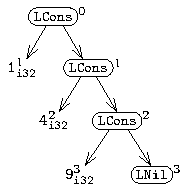
\includegraphics[scale=1.3]{chapters/figures/figExprtreeList1.pdf}}
\end{center}
\caption{\label{fig:exprtreelist}\type{List} = \cons{LNil} | \newline \cons{LCons}(\type{i32}, \type{List})}
\end{subfigure}%
&
\begin{subfigure}[b]{0.28\textwidth}
\begin{center}
{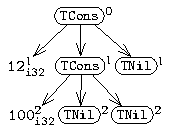
\includegraphics[scale=1.3]{chapters/figures/figExprtreeTree1.pdf}}
\end{center}
\vspace{18px}
\caption{\label{fig:exprtreetree}\type{Tree} = \cons{TNil} | \newline \cons{TCons}(\type{i32}, \type{Tree}, \type{Tree})}
\end{subfigure}%
&
\begin{subfigure}[b]{0.4\textwidth}
\begin{center}
{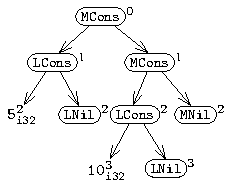
\includegraphics[scale=1.3]{chapters/figures/figExprtreeMatrix2.pdf}}
\end{center}
\caption{\label{fig:exprtreematrix}\type{Matrix} = \cons{MNil} | \newline \cons{MCons}(\type{List}, \type{Matrix})}
\end{subfigure}%
\\
\end{tabular}
\caption{\label{fig:exprtrees}Expression trees of three values, each of type \type{List}, \type{Tree} and \type{Matrix} respectively. The depths are shown as superscripts for each node in the trees.}
\end{figure}
